\documentclass[12pt, a4paper]{article}
\usepackage{verbatim} 
\usepackage{subfig}
\usepackage{wrapfig}
\usepackage{listings}
\usepackage{array}
\usepackage[utf8]{inputenc}
\setlength {\marginparwidth }{2cm}
\usepackage{todonotes}
\usepackage{newtxtext}
\usepackage{blindtext}
\usepackage{enumitem}
\usepackage{graphicx}
\usepackage{outlines}
\usepackage{pdflscape} % For landscape pages
\usepackage{float}     % For ordering images and text accordingly
\usepackage[colorlinks = true, urlcolor  = blue]{hyperref}
\graphicspath{ {./images/} }
\usepackage{biblatex}
\addbibresource{bibliography.bib}

\usepackage{hyperref}
\hypersetup{
    colorlinks=false, % Set to false if you don't want colored links
    linkcolor=blue,   % Color of links to internal documents
    filecolor=magenta, % Color of file links
    urlcolor=cyan     % Color of external links
}

\setlist[itemize]{itemsep=2pt, parsep=0pt}
\setlength{\arrayrulewidth}{0.3mm}
\setlength{\tabcolsep}{10pt}
\renewcommand{\arraystretch}{1.5}

\usepackage{xcolor}
\definecolor{light-gray}{gray}{0.95}
\newcommand{\code}[1]{\colorbox{light-gray}{\texttt{#1}}} % Functions to create code snippets with \code{code}

%\setcounter{secnumdepth}{2}

\begin{document}
\begin{titlepage}
    \centering
    \vspace*{1cm}
    
    {\Huge\bfseries DevOps, Software Evolution and Software Maintenance \par}
    \vspace{1.5cm}

    {\LARGE Group D \par}
    \vspace{1cm}
    
    {\Large Group Members: \par}
    \vspace{0.5cm}
    \begin{tabular}{rl}
        Victor Memborg-Heinrichsen & \href{mailto:vmem@itu.dk}{vmem@itu.dk} \\
        Peter Bjørholm Hansen & \href{mailto:pebj@itu.dk}{pbjh@itu.dk} \\
        Lukas Vranic & \href{mailto:luvr@itu.dk}{luvr@itu.dk} \\
        Anne-Marie Rommerdahl & \href{mailto:annro@itu.dk}{annro@itu.dk} \\
    \end{tabular}
    \vfill
    
    {\large BSc Software Development \par}
    \vspace{0.2cm}
    {\large IT University of Copenhagen \par}
    \vspace{0.2cm}
    {\large BSDSESM1KU \par}
    \vspace{0.2cm}
    {\large \today\par}
    
\end{titlepage}


\pagenumbering{arabic}
\setcounter{secnumdepth}{2}
\setcounter{tocdepth}{2}
\tableofcontents
\newpage
\pagenumbering{arabic}
\section{Process' perspective}
\subsection{Security Assessment}
To protect our system against adversaries, we first identify the assets that must be protected. We then identify which threats we could face and how. Finally, we analyze these scenarios to figure out which scenarios pose the biggest threats.

\subsubsection{Risk Identification}
Our assets:
\begin{itemize}
    \item Codebase
    \item Database
    \item Logs
\end{itemize}

Threat Sources:
\begin{itemize}
    \item SQL Injection
    \item Exposed ports (Prometheus)
    \item Vulnerable password hashing
    \item No requirements for user password (length, symbols, etc.)
    \item Vulnerable dependencies
    \item No password on Dozzle (logging)
\end{itemize}

Risk Scenarios:
\begin{itemize}
    \item A - Attacker performs SQL injection to download sensitive user data
    \item B - Attacker performs SQL injection to delete information from the database
    \item C - Attacker performs SQL injection to log in to a legitimate user's account
    \item D - Attacker brute-forces the hash of a password, letting them log in to a legitimate user's account
    \item E - Attacker uses the open ports to overload our Prometheus with queries
    \item F - Attacker intersects messages sent over the network, as they are not encrypted*** (attacker reads messages, or does man-in-the-middle to send their own messages to user)
    \item G - Attacker exploits a vulnerable dependency, which lets them perform some malicious attack. As the actual threat level depends on the specific vulnerability, we've chosen to be pessimist and assume, that the consequences will be disastrous
    \item H - Attacker accesses our logs on Dozzle, which lets them see all outputs, like usernames
\end{itemize}

\subsubsection{Risk Analysis}
Here are the scenarios presented on the risk matrix:
\begin{center}
\begin{tabular}{ |c|c|c|c|c| } 
 \hline
  & Rare & Unlikely & Likely & Certain \\ 
 \hline
 Catastrophic & B &  &  & G\\ 
 \hline
 Critical & A &  &  & \\ 
 \hline
 Marginal & &  &  F& E\\ 
 \hline
 Negligible & C &  & D & H\\ 
 \hline
\end{tabular}
\end{center}
Scenarios A, B, and C have a 'Rare' probability, as we already utilize the ORM-library 'GORM'. GORM uses prepared statements and automatically escapes arguments to avoid SQL injection. Without GORM, the probability would be much higher.\\
Scenario F was dealt with using the TLS protocol. Our Minitwit application using TLS is hosted at https://lukv.dk.\\
For scenario G, we have added Dependabot, which will automatically search for outdated dependencies, and create pull requests to update such dependencies.
\\\\
\\
For scenario E, we would have to perform a workaround, as the exposed ports are caused by Docker and UFW being incompatible, an issue which has not yet been patched. However, Prometheus is the only service that is exposed, and the only threat is Prometheus crashing due to an overload of queries. Therefore, it is not considered a high-priority threat.
\\\\
\\
Scenario H can be prevented by locking our Dozzle interface with a password. However, no sensitive data is logged in Dozzle, and thus it is considered low priority.

\subsection{Scaling and Upgrades}
\subsubsection{Scaling}
To scale our Minitwit application, we performed horizontal scaling using Docker Swarm. We created three manager nodes and four worker nodes. \\
We have replicas of the following services:
\begin{center}
\begin{tabular}{ |c|c|c| } 
 \hline
 Service & Replicated/Global & No. of replicas \\ 
 \hline
 Minitwit App & Replicated & 3 \\ 
 \hline
 Minitwit API & Replicated & 4 \\
 \hline
 Prometheus & Global & N/A \\ 
 \hline
 Dozzle & Global & N/A \\ 
 \hline
\end{tabular}
\end{center}

Prometheus and Dozzle are set to be global services, meaning that one instance of each runs on every node in the swarm. This ensures that monitoring and logging are consistently performed on all nodes, preventing any loss of critical information, whether it is logging or monitoring, due to missing coverage.

\subsubsection{Upgrades}
We use a rolling update strategy with a start-first-order to update the services in our swarm. This means that one replica at a time is updated by starting a new container before stopping the old one, ensuring minimal downtime. Updates are monitored for 30 seconds, and if any failures are detected, our swarm will automatically roll back to the previous working version \cite{dockerComposeDeploy}.

\subsection{CI/CD Chain}
We are using GitHub Actions to automate the testing and deployment of Minitwit. There are 5 GitHub Actions workflows:

\begin{outline}[enumerate]
    \1 Deploy services to DigitalOcean
        \2 Runs when there is a push to \code{main}.
        \2 This workflow builds and pushes Docker images to Docker Hub, it then pulls them onto to the server on DigitalOcean.
    \1 Run tests and linter
        \2 Runs on any push or when a PR is updated/created.
        \2 Runs linters and tests on new commit or PR.
    \1 Release MiniTwit
        \2 Runs every thursday at 23:30 UTC.
        \2 Creates a weekly release of MiniTwit.
    \1 Run linter
        \2 Runs when called by other workflows.
        \2 Lints Go files using golangci-lint.
    \1 Hadolint on dockerfiles
        \2 Runs when called by other workflows.
        \2 Lints Docker files using Hadolint.
\end{outline}
\begin{figure}[H]
    \centering
    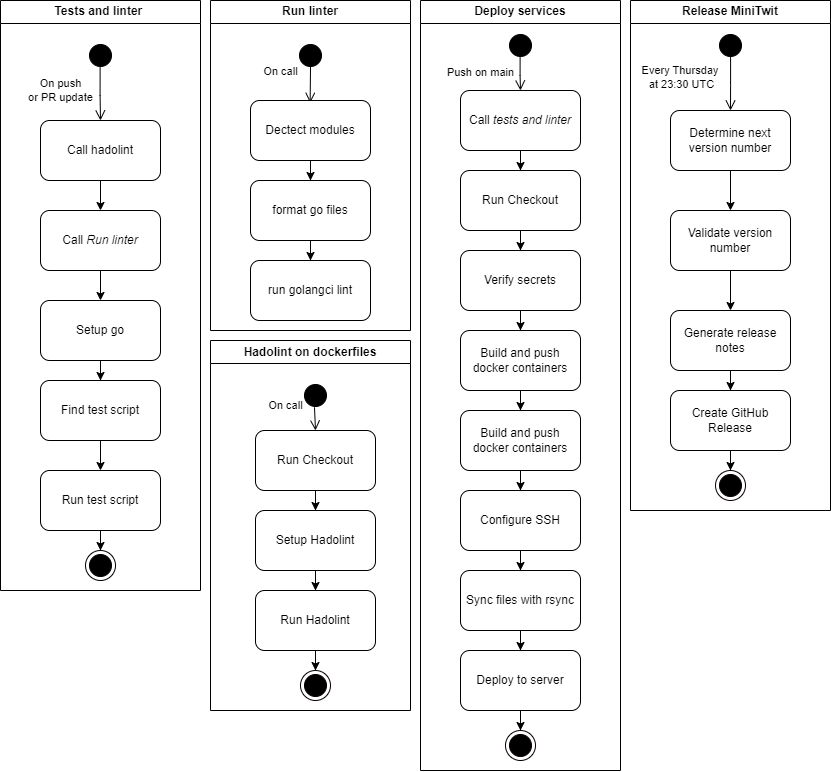
\includegraphics[width=\textwidth]{images/Worflows.png}
    \caption{Activity diagram of the workflows.}
\end{figure}


\subsection{Monitoring}
We monitored MiniTwit using Prometheus for collecting metrics and Grafana for visualizing them. This setup provided great insights into the application's performance and behavior.

\subsubsection{Prometheus}\label{prom}
Prometheus was integrated into both the API and the application through a custom middleware that intercepts HTTP requests to gather metrics. The metrics collected includes:

\begin{itemize}
\item \texttt{http\_requests\_total}: A counter that counts the total number of HTTP requests. It includes labels for request path, HTTP method, and status code. This metric helped us monitor request load per endpoint, track response statuses (in general or just on an endpoint basis).
\item \texttt{http\_request\_duration\_seconds}: A histogram measuring the time taken to process HTTP requests, in seconds. It is labeled by request path and method, enabling performance benchmarks for endpoints.
\item \texttt{http\_response\_messages\_total}: A counter that logs the total number of HTTP responses, categorized by status code and message type. Before logging was fully implemented, this metric was particularly helpful in identifying which endpoints triggered specific status messages and understanding the reasons behind them. A bit deprecated as soon as logging was implemented.
\end{itemize}

Seen in retrospect, it would have been a good idea also to collect metrics on database queries, but this will be described more thoroughly in section \ref{maintainence}

\subsubsection{Grafana}
Althoughugh Prometheus was important for collecting data, Grafana is utilizto visualize the data. Grafana connects to Prometheus as a data source, enabling the creation of dashboards. As mentioned in section \ref{prom} we monitored both our API and app, which resulted in us setting two dashboard up; one for the app and one for the API.
\\\\
For instance, the API dashboard converted the metrics collected by Prometheus into a clear visual representation of the API's health and performance. Panels were set up to showcase:
\begin{itemize}
    \item Indicators from \texttt{http\_requests\_total}, such as the rate of requests per second, overall request load distributed by endpoint, and the ratio of successful and client-error status codes.
    \item Performance monitored by \texttt{http\_request\_duration\_seconds}, including average response times and 99th percentile latency, allowing for quick identification of performance degradation.
\end{itemize}

\subsection{Logging}
Logging in MiniTwit was implemented using Dozzle. When we initially wanted to implement logging, we implemented an ELK stack in our standard Docker Compose. This was a very basic implementation with no parsing or user setup. However, this never made it to production because while it was being worked on, we implemented Docker Swarm, and suddenly, a lot changed for our system. Meanwhile, another group member noticed a TA proposing a look at Dozzle if you had problems with ELK. Dozzle was implemented with great success in no time and worked great for us.

\subsubsection*{What do we log in Minitwit?}
In Minitwit, we log application events using Go's standard logging functions, including error messages from our main application and API services. Our database layer (GORM) is configured to log at a warning level. We also log API error responses and critical application failures.

\subsubsection*{How do we aggregate logs?}
All logs in Minitwit are aggregated at a container level using Docker’s built-in logging, with every service writing to \texttt{stdout} and \texttt{stderr}. We use Dozzle, deployed in global mode in our swarm, to view and search logs from all running services in real time through its web interface. 

\subsubsection*{Why we choose Dozzle}
We ended up using Dozzle because it enabled us to filter logs by container and log level. We can transmit logs from our services in real time and filter them by service and different logging levels. A sidebar is available, which is equipped with a fuzzy search ability and provides a comprehensive overview of each service, node, replica, and swarm manager. It offers a standard search within the logs for manual searches and the ability to conduct Regex searches within the logs. Dozzle is a simple and effective method of logging, as it is not infrastructure-intensive and is extremely lightweight. Implementation within a Docker swarm is effortless with Dozzle. Dozzle was the optimal choice for us due to its user-friendly interface and all of the aforementioned.

\subsubsection*{ELK stack features we missed out on}
We cannot implement a role-based access control or authentication system with Dozzle, which is unsuitable for production. As of now, unauthorized users can see our logs, and that is, as mentioned, potentially a security breach. We cannot save our logs indefinitely, and cannot distinguish between what should be parsed and what should not. Additionally, we are forfeiting the performance that Elasticsearch would have offered through its robust indexing and search capabilities.
\\\\
While there is a lot more we miss out on not using an ELK stack, these are the ones we feel were relevant to us. An ELK stack would require much more management, and you could almost endlessly improve it. We feel that Dozzle provided us with what we needed. Combined with our monitoring, we have the opportunity as developers to quickly gain an overview of bottlenecks or bugs in the application and fix them accordingly. 

% Print the bibliography
\printbibliography
% \newpage
% \input{sections/apendix}
\end{document}